\chapter{Systematic Uncertainty}
In this chapter the systematic errors of the analysis are discussed. These uncertainties arise due to various reasons, some of them being the difference between real and simulated data, or due to the nature of the approaches taken in a specific analysis. Depending on their type, some uncertainties are generic and prepared beforehand in order to be used in all analyses, while others are analysis specific and possible sources need to be thought through thoroughly. 

\section{PID efficiency correction}

The PID cut efficiency for the three charged particles in our signal decay needs to be corrected on MC due to various differences when comparing to data. The Belle PID group has prepared correction factor and systematics tables for PID cut efficiencies of all charged particles. In case of kaon ID and lepton ID, the tables are binned in experiment numbers, particle momentum and in $\cos\theta$ of the particle, where for each bin a ratio of efficiencies between MC and data is provided, as well as the systematic errors. Each particle's correction factor and error is shown in Table \ref{tab:PID}, as well as the corresponding entry for all 3 particles. The entries are shown for both the signal and control region.

The central values were obtained with a weighted average over all experiments, where $100\%$ correlation for error calculation was assumed. Full correlation was also assumed when calculating the $KK$ correction, as both $K$ use the same PID information.

\begin{table}[H]
	\centering
	\begin{tabular}{|l|c|c|}
		\hline
		PID correction and systematics & Control region & Signal region \\
		\hline
		Same sign $K$ (w.r.t the $B$) & $1.005\pm 0.009$ & $1.007\pm 0.010$\\
		\hline
		Opposite sign $K$ (w.r.t the $B$) & $1.004\pm 0.009$ & $1.006\pm 0.009$\\
		\hline
		$e$ & $0.977\pm 0.011$ & $0.976\pm 0.011$\\
		\hline
		$\mu$ & $0.985\pm 0.009$ & $0.980\pm 0.009$\\
		\hline
        $\ell$ & $0.981\pm 0.007$ & $0.980\pm 0.007$\\
		\hline
		\hline
		$KKe$ & $0.986 \pm 0.021$ & $0.988\pm 0.022$\\
		\hline
		$KK\mu$ & $0.994 \pm 0.020$ & $0.993\pm 0.021$\\
		\hline
		$KK\ell$ & $0.990 \pm 0.019$ & $0.990\pm 0.020$\\
		\hline
	\end{tabular}
	\caption{PID correction factors and systematic error for various charged particles and their combinations.}
	\label{tab:PID}
\end{table}

\section{Toy MC experiments}

Toy MC experiments allow us to study the yields, errors and the pulls of the signal fit by generating our own pseudo datasets, according to the MC, and not producing it in the standard way, which consumes unaffordable amounts of CPU time. In order to test the fit behavior, a toy MC study was performed where all available MC was used for template creation. 

\subsection{Pseudo experiments for expected signal yield}

We constructed $3\E{3}$ pseudo datasets, where each dataset was generated with the expected amount of each template category, distributed according to the Poisson distribution. All fits were performed with the optimal initial uniform binning of $20\times20$ bins in \vars.

%Figure \ref{fig:toyMC} shows distributions of the fit yields, errors and the pull distribution of all pseudo fits. The fits seem to be under control, although there is a slight bias present of about $N = #, and the pulls follow a normal distribution with a mean of $(1.1\pm1.8)\E{-2}$ and standard deviation of $(1.013\pm0.013)$. The mean ($\bar X$) and the standard deviation $(S)$ were calculated in the usual way, while the errors of these statistics were obtained by calculating the standard error of the mean ($\sigma_{\bar X}$) and standard deviation ($\sigma_S$), taken from \cite{ahn2003standard}, as
%\begin{equation}
%\sigma_{\bar X} = \frac{S}{\sqrt{N}},\quad \sigma_{S} = \frac{S}{\sqrt{2(N-1)}},
%\end{equation}
%where $N$ is the number of performed measurements.

\begin{figure}[!htbp]
	\centering
	\captionsetup{width=0.8\linewidth}
	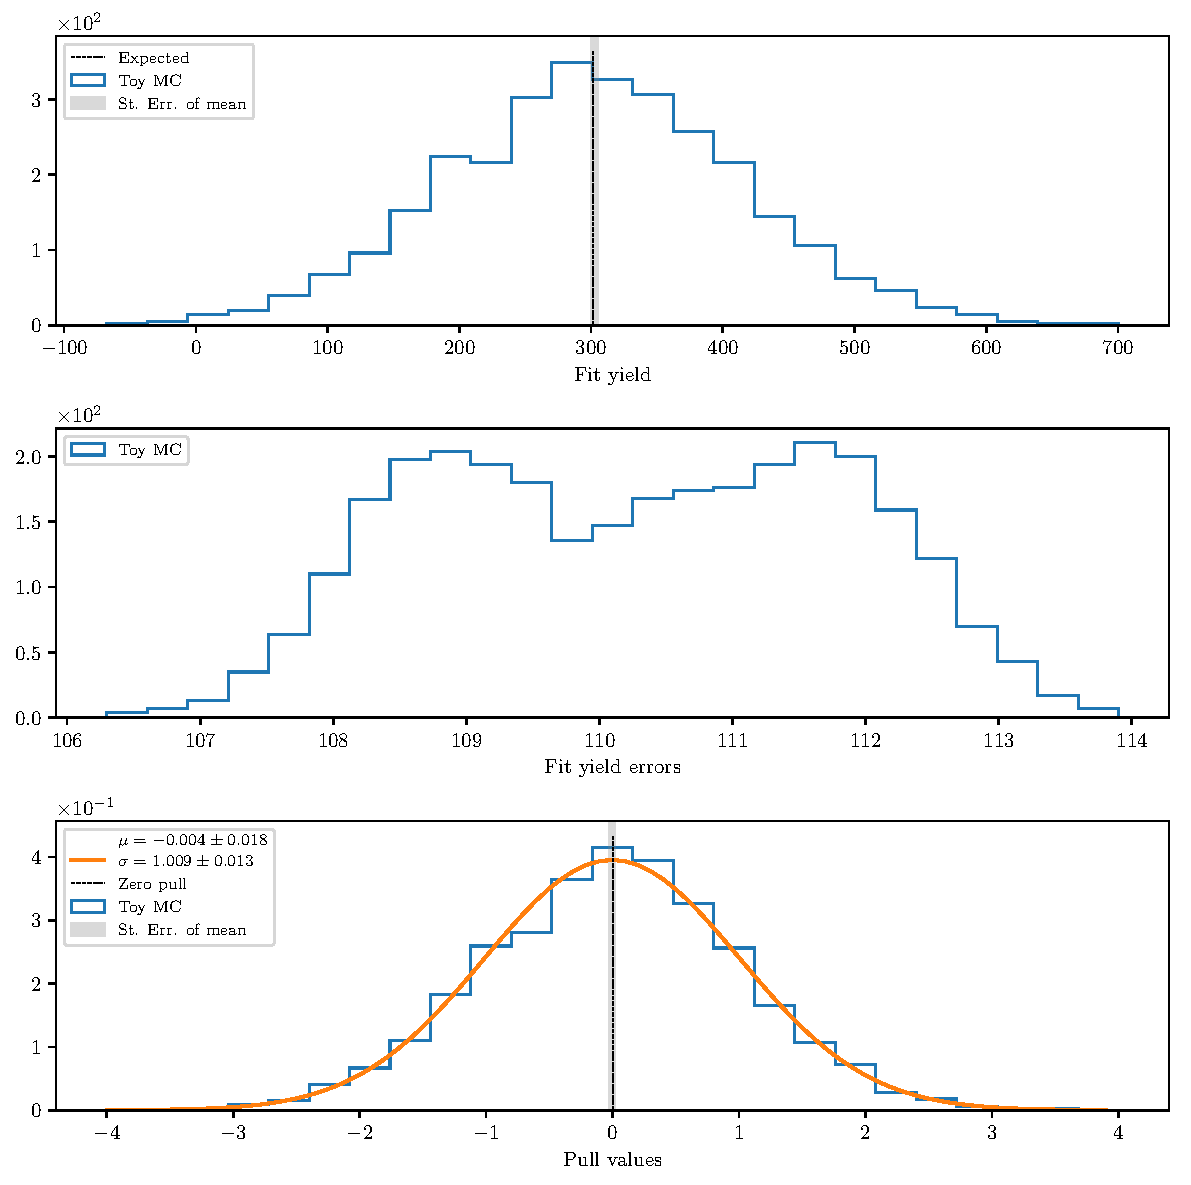
\includegraphics[width=\linewidth]{fig/toyMC}
	\caption{Toy MC fits of pseudo data showing the fit yield (top), fit errors (center) and the pull distribution of the fits (bottom).}
	\label{fig:toyMC}
\end{figure}

\subsection{Pseudo experiment linearity test}
Linearity test is used for determining sensitivity of the fit to the amount of signal in the fitted sample. Since this is a first measurement of this decay channel, MC modeling is not reliable and could be very different from reality, so we need to perform this test in order to determine our sensitivity to smaller, as well as larger amounts of expected signal.

The pseudo datasets are generated in the same way as in the previous subsection, with the exception of signal, which is generated with various amounts. $50$ steps from $[0.1,~10]$ in the logarithmic scale are taken for fractions of signal amount and for each fraction we generate 500 pseudo datasets according to Poisson statistics.

Figure \ref{fig:lin_test} shows the mean fit yield and expected yield difference, mean pull and the mean significance at each signal fraction value. The expected MC result is shown at fraction value $1$. The plots show no significant bias with with respect to the signal fraction, while the pulls seems to be described by the normal distributions throughout the fraction range. At expected value we are at about $3.2\sigma$ significance, as already pointed out at the beginning of this section.

\begin{figure}[!htbp]
	\centering
	\captionsetup{width=0.8\linewidth}
	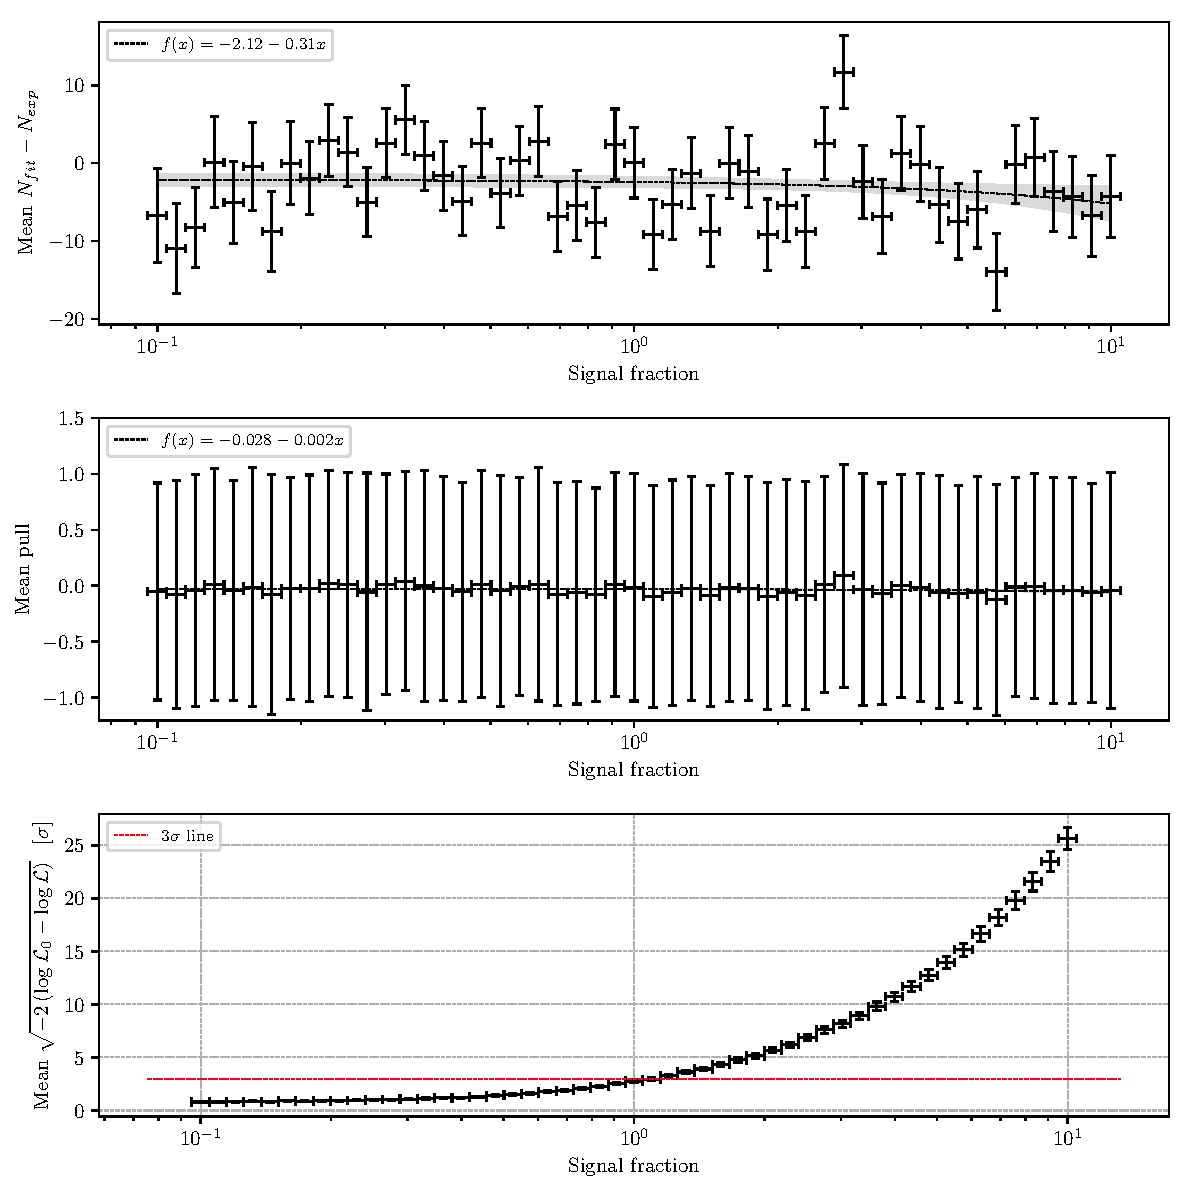
\includegraphics[width=\linewidth]{fig/lin_test}
	\caption{Mean fit yield and expected yield difference (top), mean pull (center) and mean significance (bottom) as a function of signal fraction.}
	\label{fig:lin_test}
\end{figure}



\section{Fit Bias}
Signal and background templates in our analysis are not perfectly distinct from one another and may potentially cause some over- or underestimation of the signal fit yield. In order to study this problem, we estimated the fit bias as a function of the signal yield in the form of a linear approximation, as already shown in Figure X. The bias function is approximated as
\begin{equation}
bias function,
\end{equation}
which leads to a systematic uncertainty of about X at the value of expected signal yield.


\section{Fit Template Smearing and Offset}


\section{Effects of a Finite MC sample}
The shape of signal and backgrounds templates in our analysis is fixed and only their normalization is considered in the fit. Due to the finite size of the MC sample, the template shape introduces an additional source of uncertainty, as it may differ if produced in a separate, equal-sized MC sample. Since the bins in these 2D histogram templates are statistically independent, we can take each bin and vary the bin content according to the Poisson distribution. This procedure is repeated for X times and the width of the fit yield distribution, shown in Figure X, is taken as the uncertainty estimate.

\section{MVA Selection Efficiencies}


\section{Model Uncertainty Effects}
The used signal decay model in the generation step was \texttt{ISGW2} [X], which is known not to be the most precise model for such decays (which ones X)? Due to this uncertainty, our analysis has been made as model independent as possible via means of not using variables, which might have a model dependent nature, in any kind of selection steps or MVA trainings. Such variables are i.e. squared momentum transfer to the lepton pair ($q^2$), invariant mass of the two kaon daughters ($m_{KK}$) or decay angle between any two charged particles in the final state.

In order to test the effects of model uncertainty on our final result, we prepare two additional signal MC samples, produced with an extreme scenario decay model. In the first scenario we generate the signal MC sample with a generic phase-space decay mode \texttt{PHSP} [X], which results in continuum-like distributions of $q^2$ and $m_{KK}$. In the other scenario only resonant-like contributions in $m_{KK}$ are used. These two scenarios act as extreme cases of decay model choice and present a reasonable measure of the model uncertainty. Figure X shows the generated $m_{KK}$ distribution of the three mentioned decay models and distributions of \vars~after the final selection. The different signal templates are used and the range of the corresponding fit yields is taken as the uncertainty range.

PLOTS AND MORE TEXT

\section{Summary of Systematics}





